\begin{figure}[!t]
    \centering
    \vspace{-0.1in}
    \makebox[\textwidth][c]{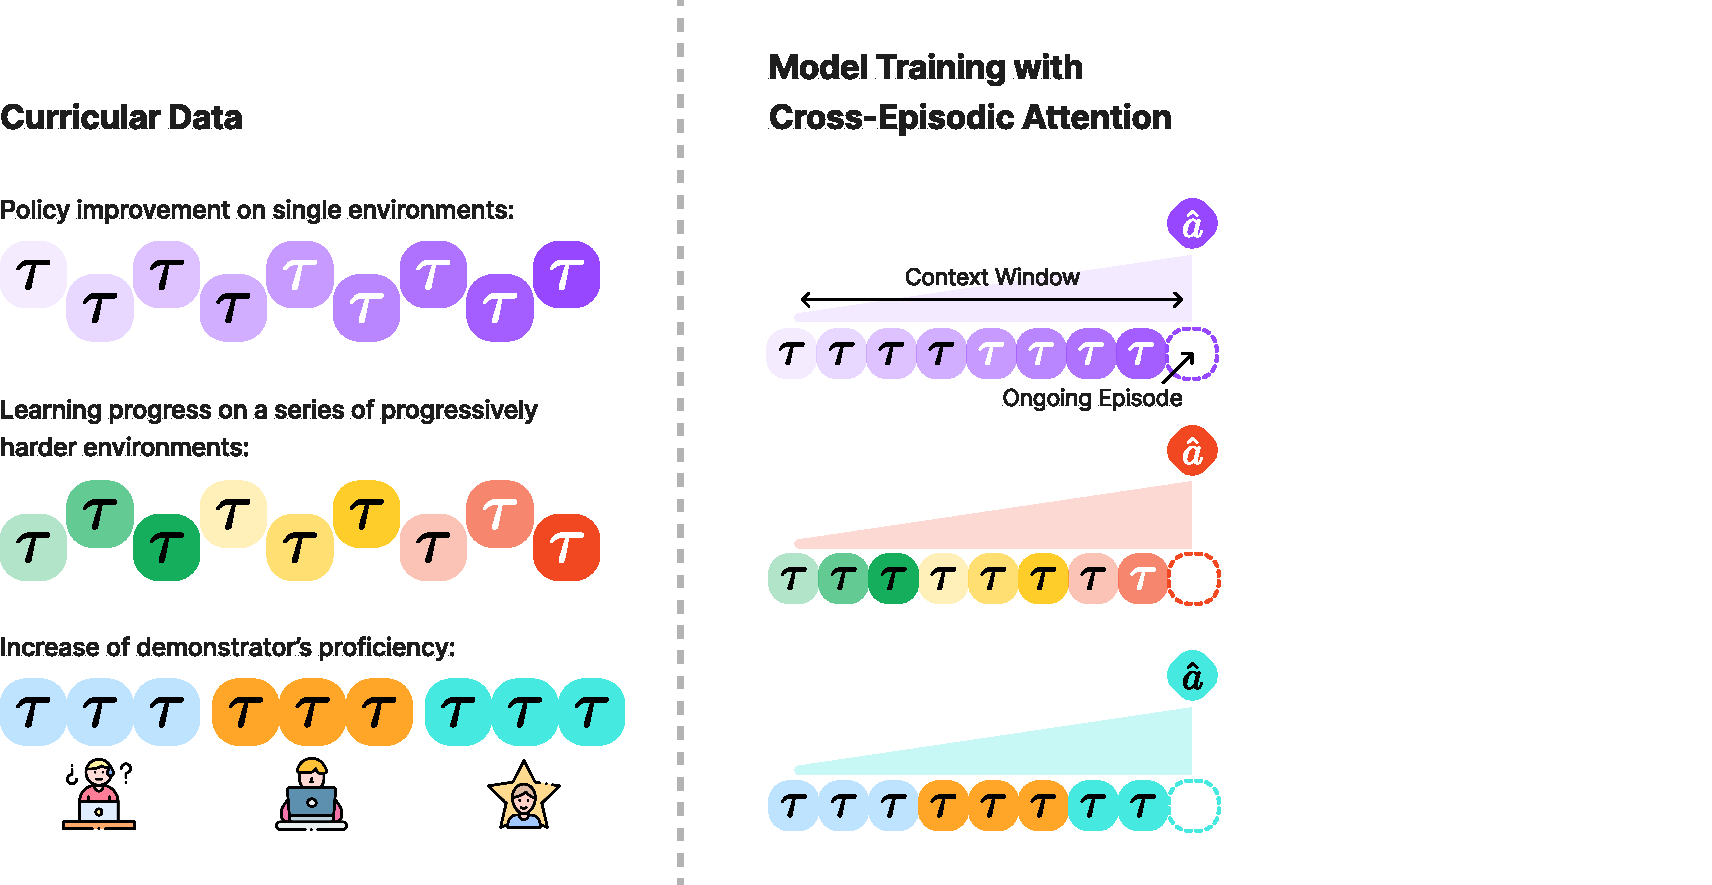
\includegraphics[width=0.9\textwidth]{fig/pull_fig-fig.pdf}}
    \caption{\textbf{Cross-episodic curriculum for Transformer agents.}
    \cec involves two major steps:
    \textit{\mbox{1) Preparation of curricular data.}} We order multiple experiences such that they explicitly capture curricular patterns. For instance, they can be policy improvement in single environments, learning progress in a series of progressively harder environments, or the increase of the demonstrator's expertise.
    \textit{2) Model training with cross-episodic attention.} When training the model to predict actions, it can trace back beyond the current episode and internalize the policy refinement
    for more efficient learning.
    Here each $\tau$ represents an episode (trajectory). $\hat{a}$ refers to actions predicted by the model.
    Colored triangles denote causal Transformer models.
    }
    \label{fig:pull_fig}  
\end{figure}

